%========================================================================
% Modelo para elaboracao de textos academicos: TCC, dissertacoes e teses
% Elaborado pelo GISIS - Grupo de Imageamento Sismico e Inversao Sismica.
%========================================================================
\chapter{Metodologia}
\label{ch:metodologia}


\section{Construção dos modelos de velocidade}

\begin{figure}[H]
	\centering
	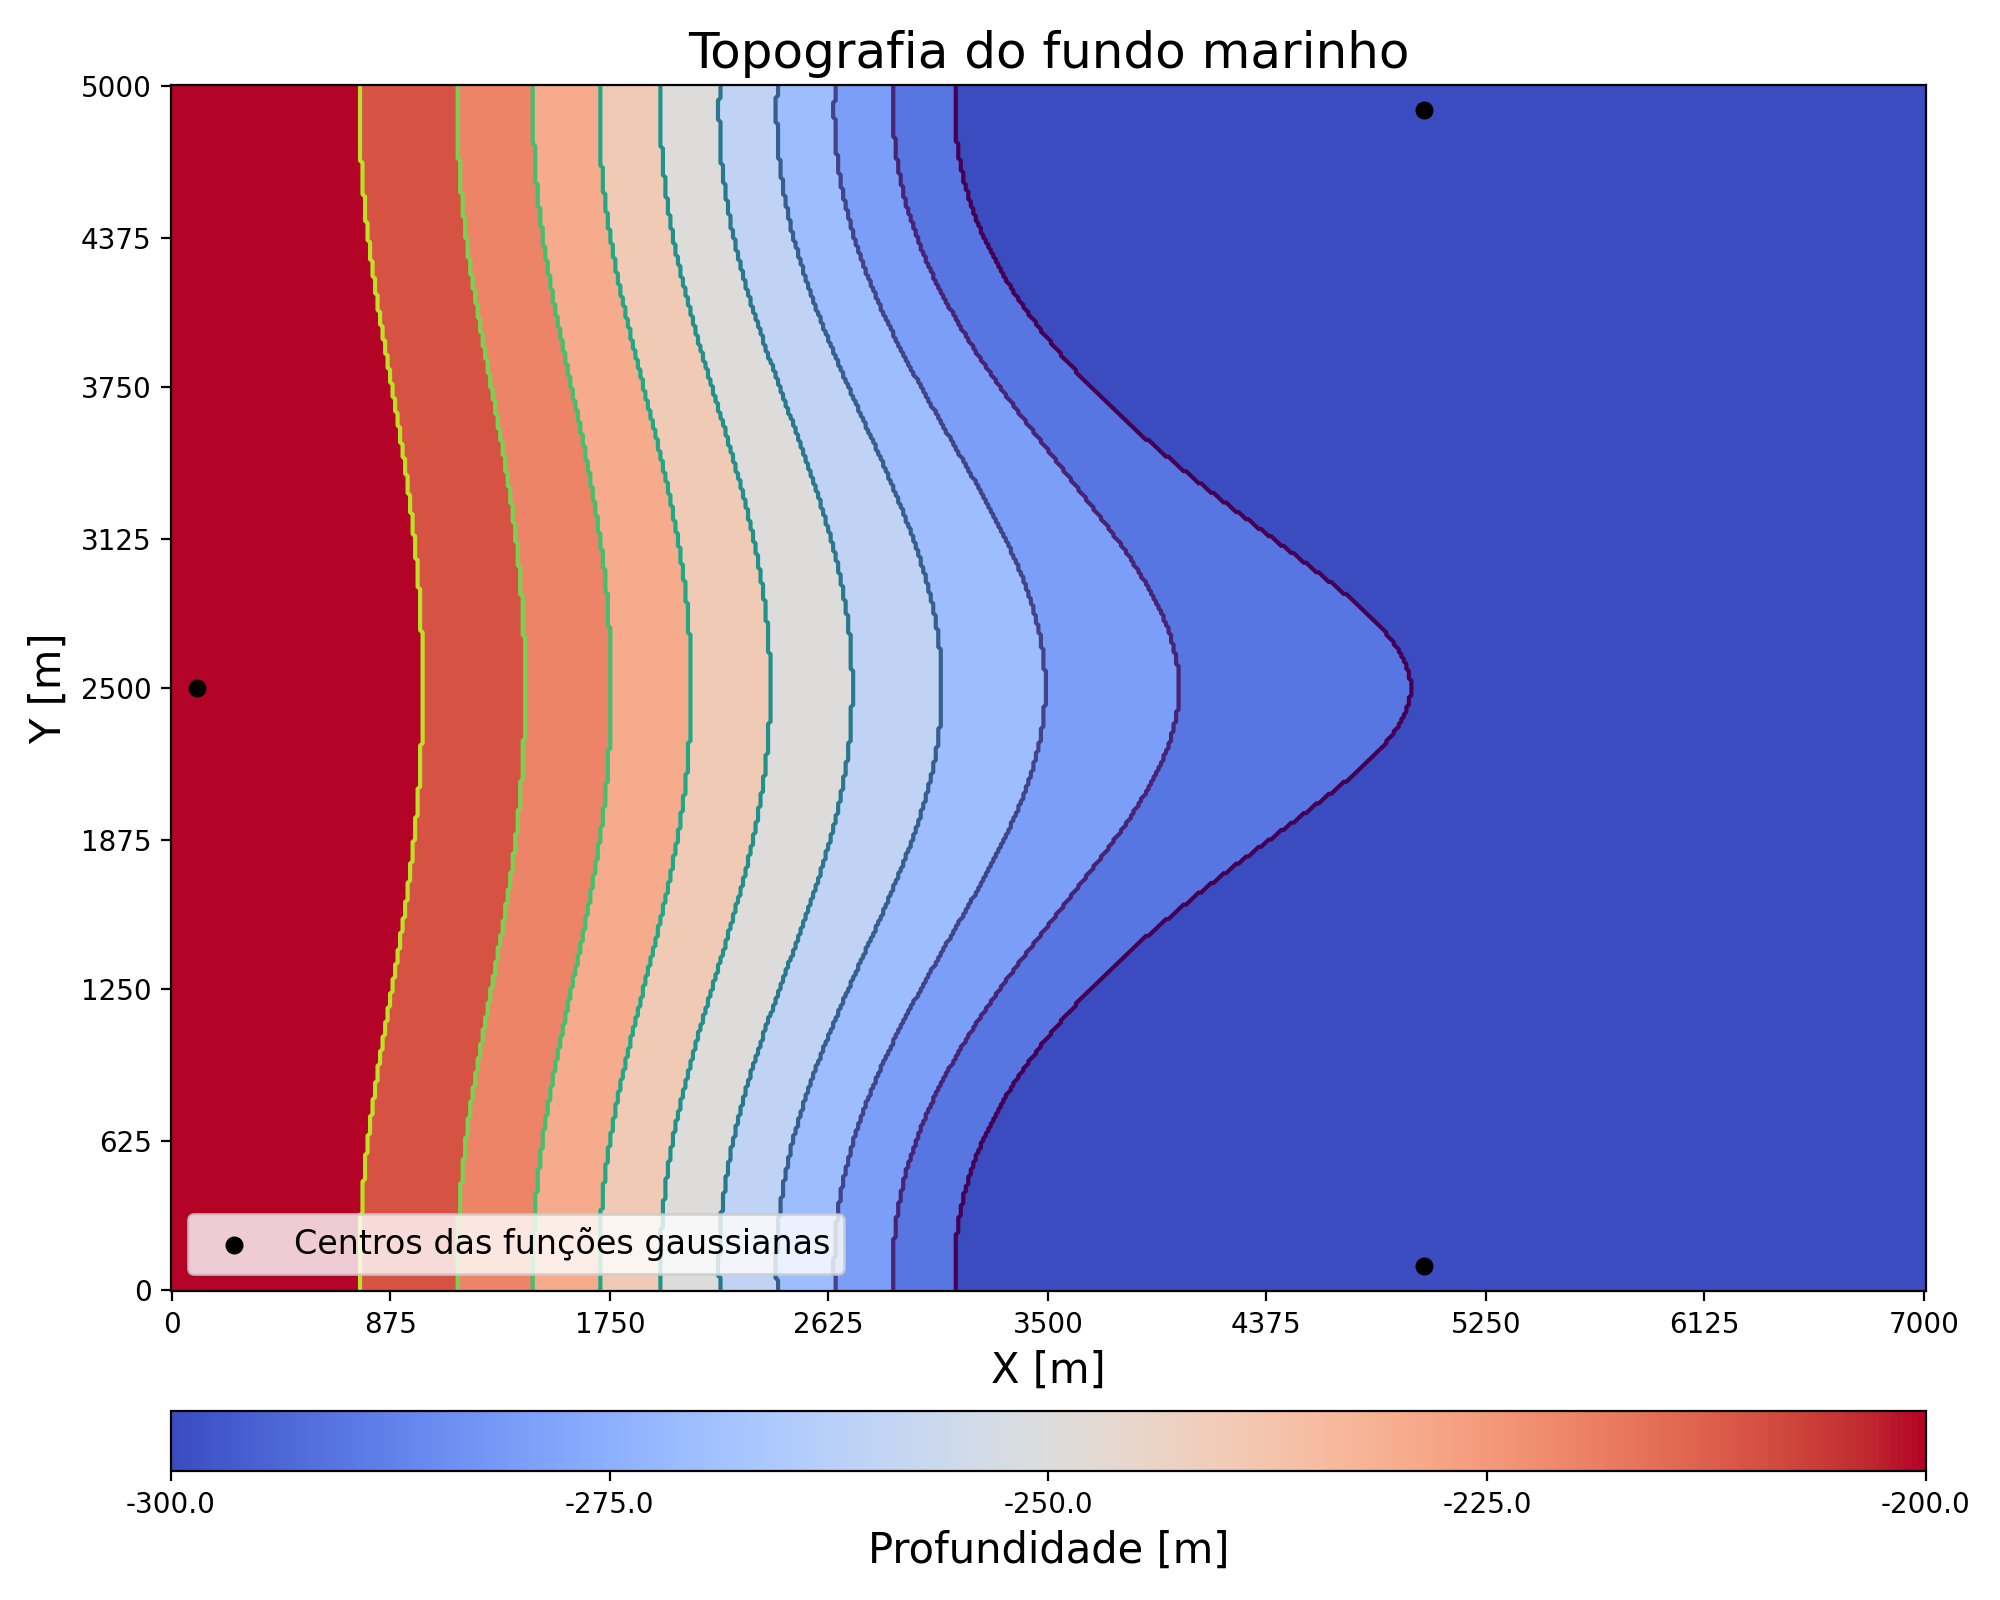
\includegraphics[width=11cm,height=8cm]{Imgs/Metodologia/water_bottom_surface_gaussian.png}
	\caption{Superfície do fundo marinho com o posicionamento dos centro das gaussianas aplicadas. Elevação predominantemente entre 300 e 200 m de profundidade.}
	\label{fig:water_bottom_surface_gaussian}	
\end{figure}


\begin{figure}[H]
	\centering
	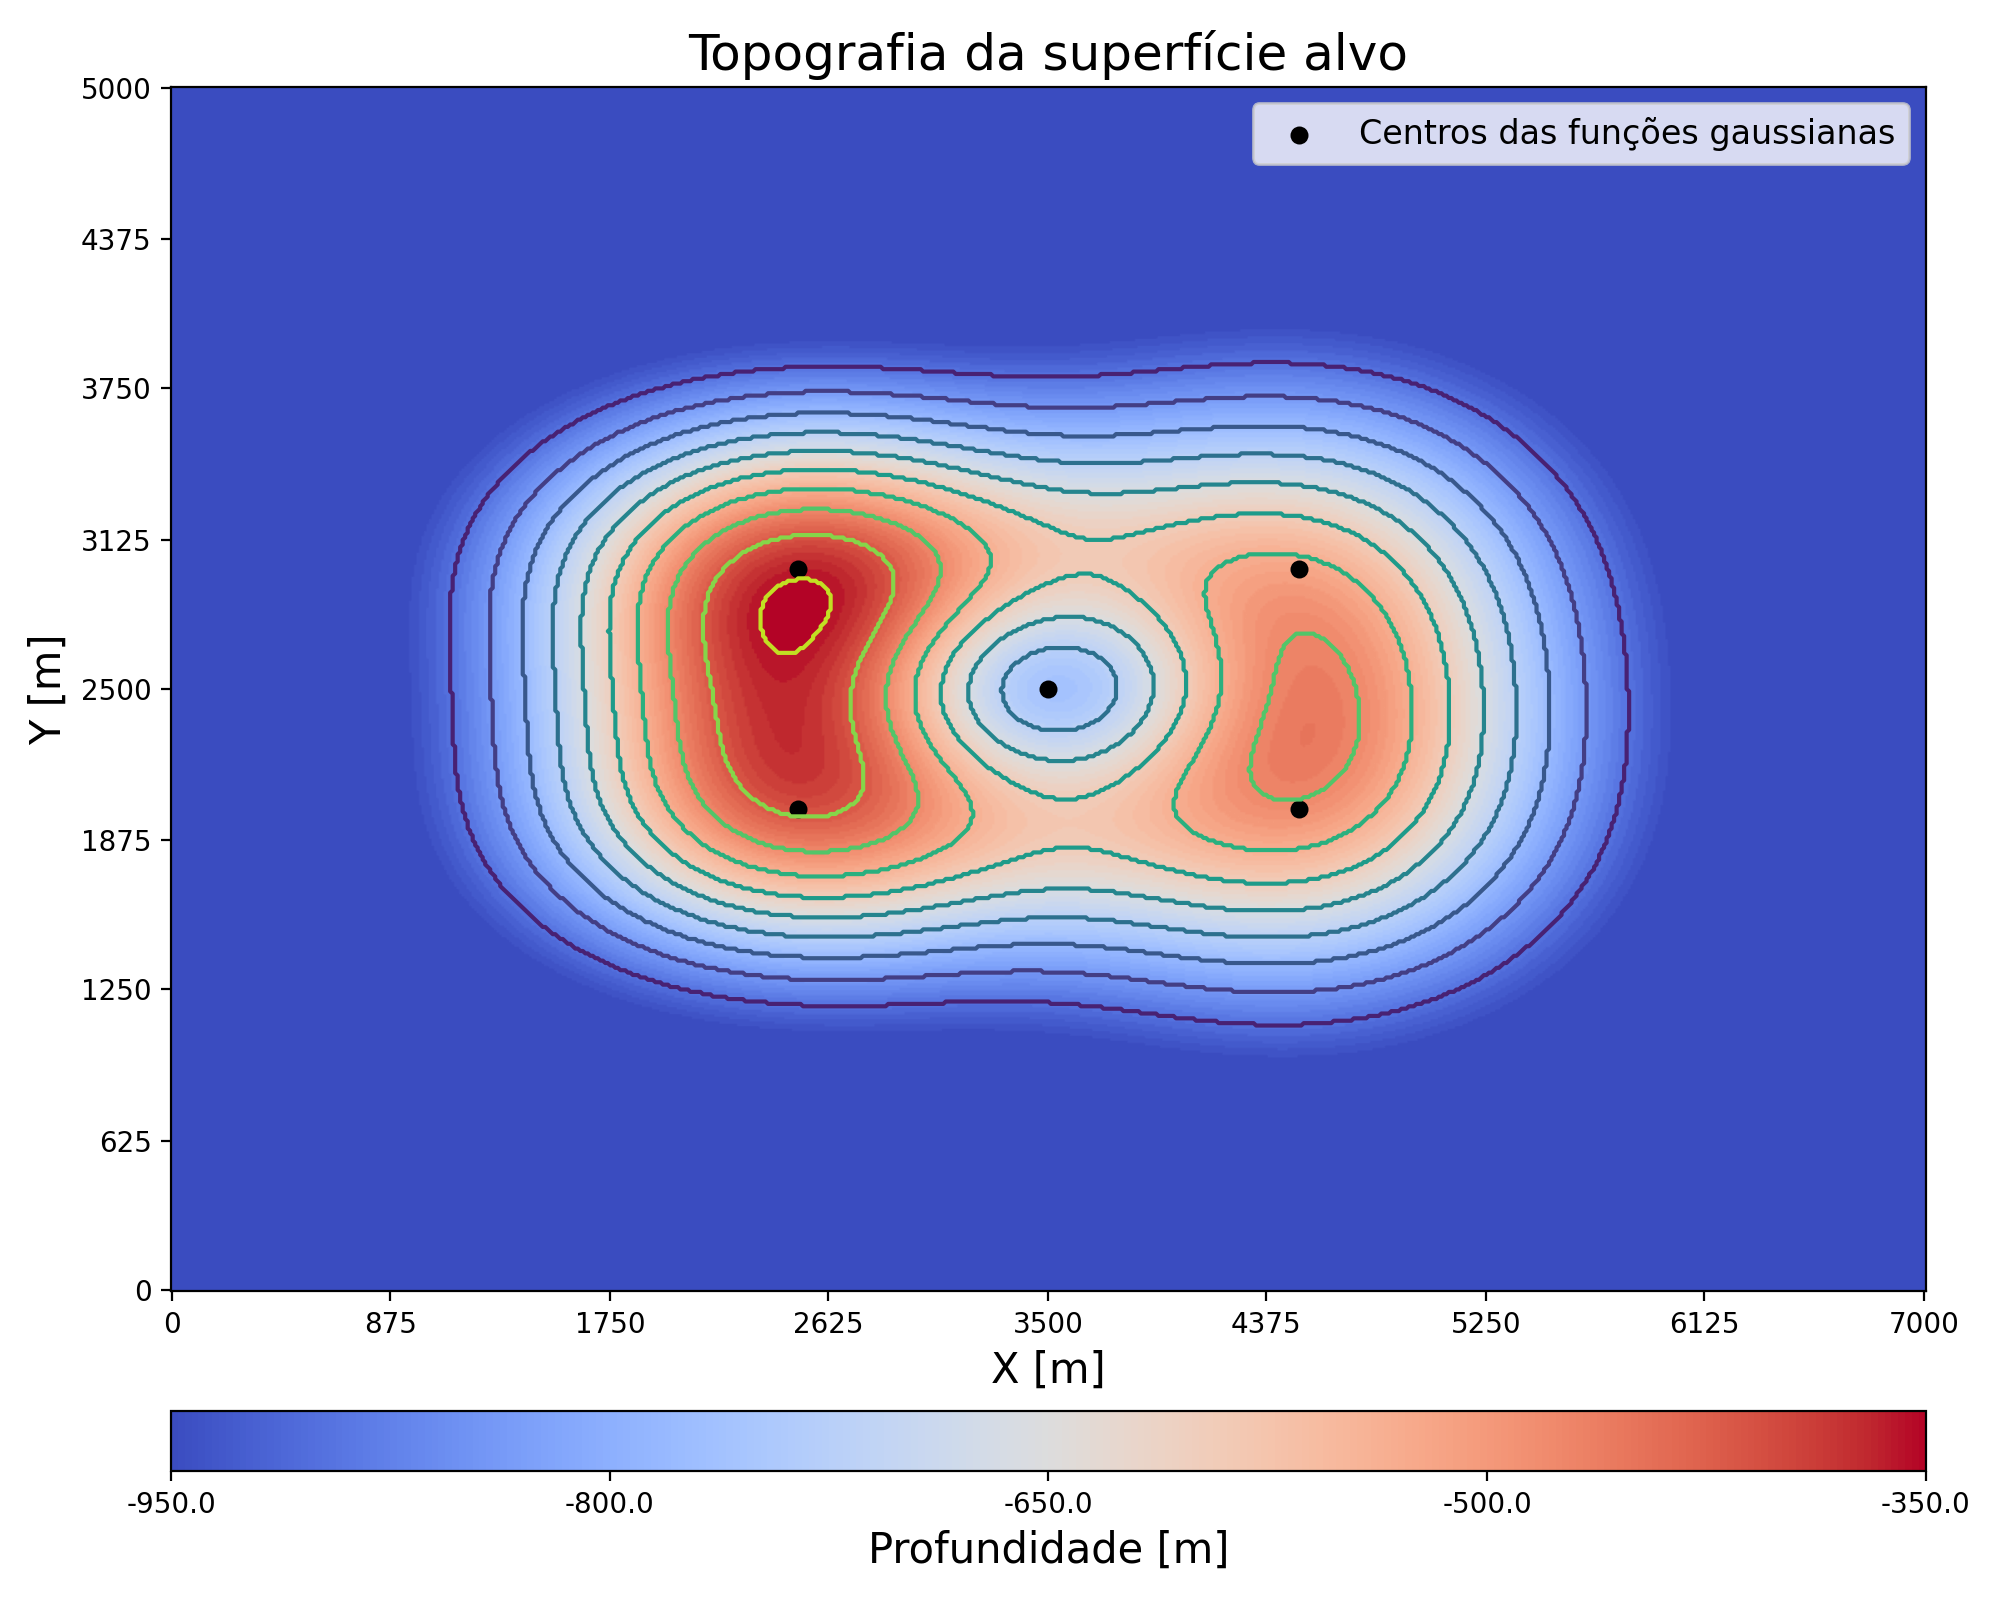
\includegraphics[width=11cm,height=8cm]{Imgs/Metodologia/target_surface_gaussian.png}
	\caption{Superfície alvo com o posicionamento dos centros das gaussianas aplicadas. Elevação entre 950 e 350 m de profundidade.}
	\label{fig:target_surface_gaussian.png}	
\end{figure}


\begin{figure}[H]
	\centering
	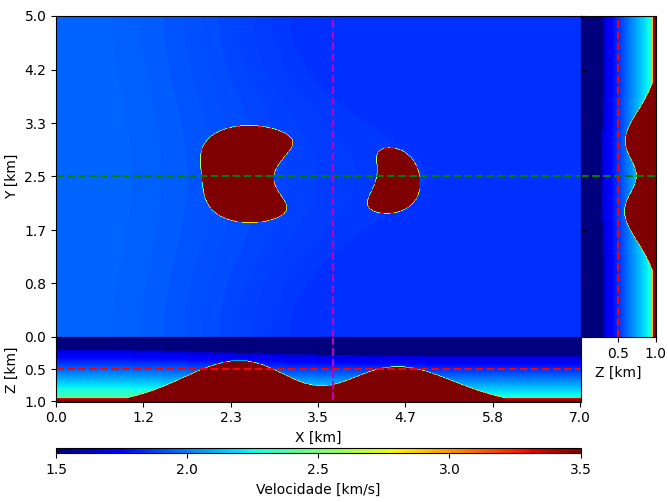
\includegraphics[width=12cm,height=9cm]{Imgs/Metodologia/true_model.png}
	\caption{Modelo de referência para gerar o dado observado. Variação de velocidade entre 1500 e 3500 m/s. Tentativa de simulação com altos contrastes de velocidade.}
	\label{fig:true_model}	
\end{figure}


\begin{figure}[H]
	\centering
	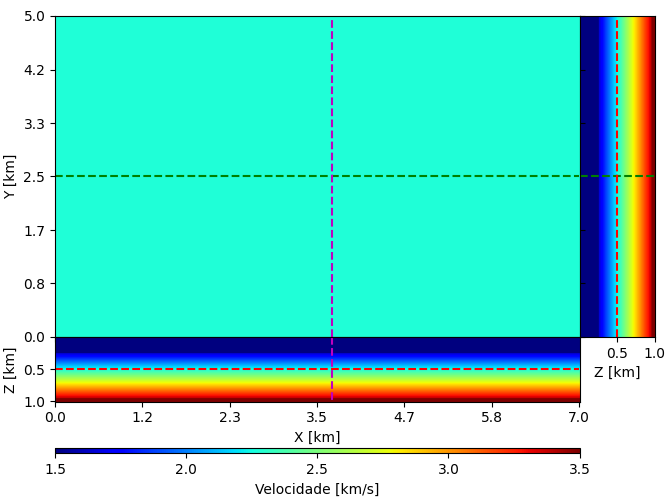
\includegraphics[width=12cm,height=9cm]{Imgs/Metodologia/init_model.png}
	\caption{Modelo base para inicializar o processo tomográfico. Simulação de camadas plano paralelas com baixos contraste de velocidade seguindo uma equação de gradiente linear com a profundidade.}
	\label{fig:init_model}	
\end{figure}




\section{Geometria de aquisição}

\begin{figure}[H]
	\centering
	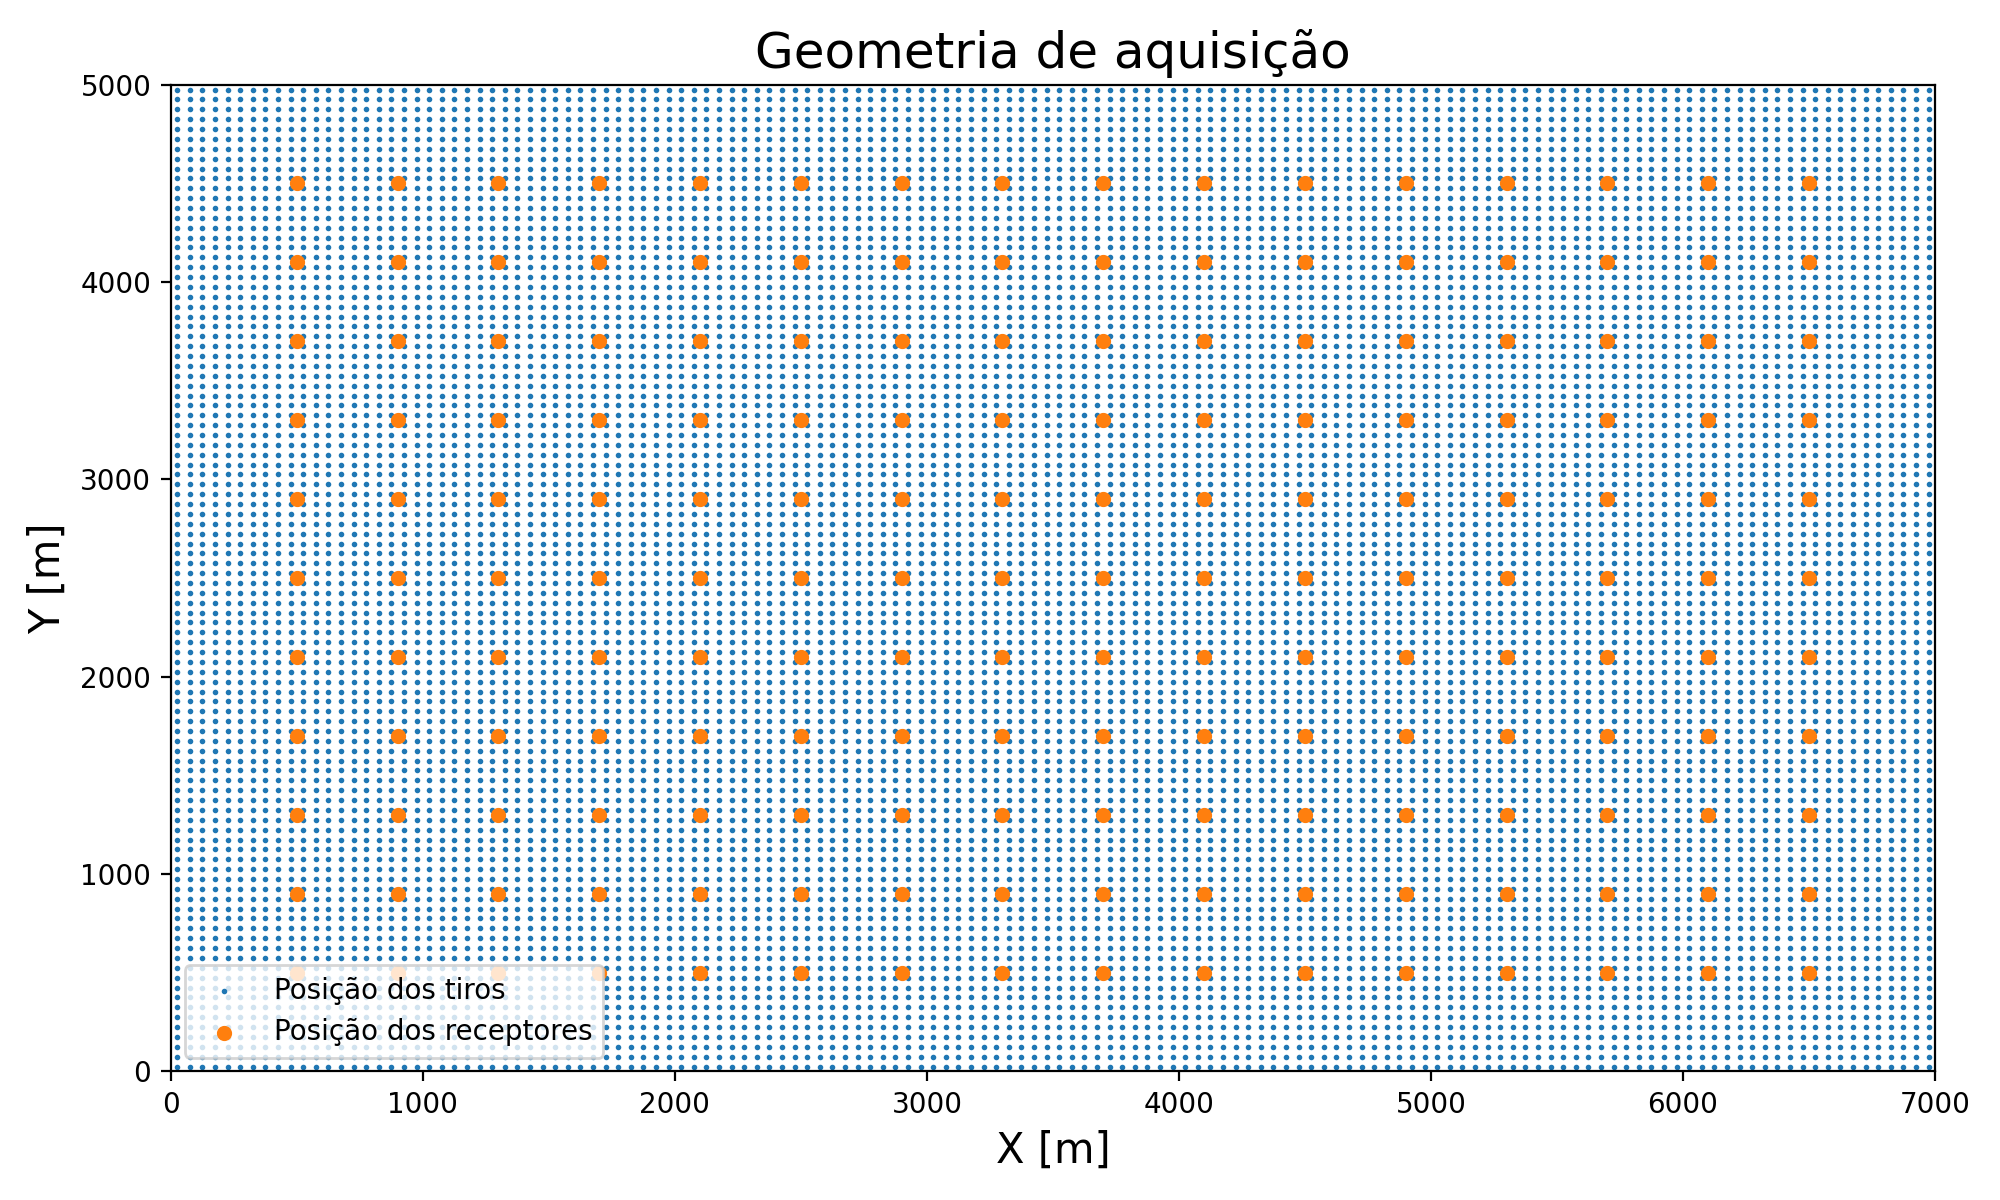
\includegraphics[width=12cm,height=7cm]{Imgs/Metodologia/complete_geometry.png}
	\caption{Configuração da geometria completa de aquisição contendo 176 receptores localizados no fundo marinho e 14000 tiros na superfície do oceano. Foi considerado 50 m para o espaçamento entre tiros e 400 metros para os receptores em ambas direções X e Y.}
	\label{fig:complete_geometry}	
\end{figure}


\begin{figure}[H]
	\centering
	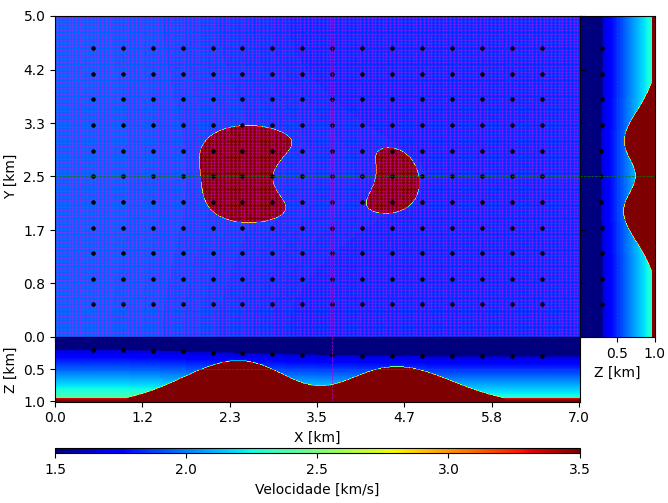
\includegraphics[width=12cm,height=9cm]{Imgs/Metodologia/true_model_geometry.png}
	\caption{Geometria de aquisição projetada no modelo de referência.}
	\label{fig:true_model_geometry}	
\end{figure}


\begin{figure}[H]
	\centering
	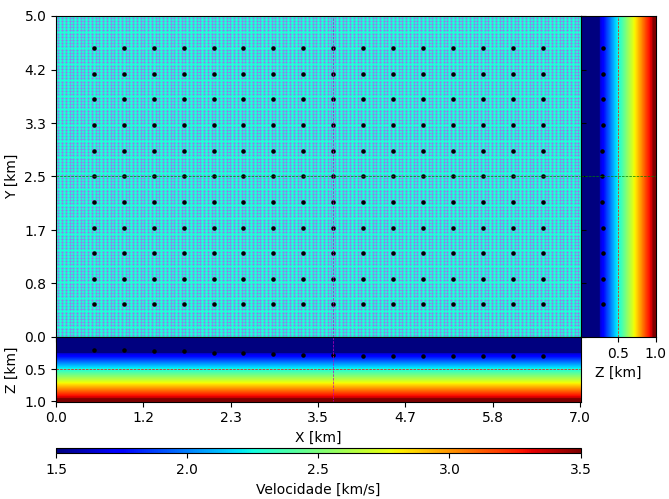
\includegraphics[width=12cm,height=9cm]{Imgs/Metodologia/init_model_geometry.png}
	\caption{Geometria de aquisição projetada no modelo inicial.}
	\label{fig:init_model_geometry}	
\end{figure}




\section{Dado observado sintético}


\begin{figure}[H]
	\centering
	\subfloat[]{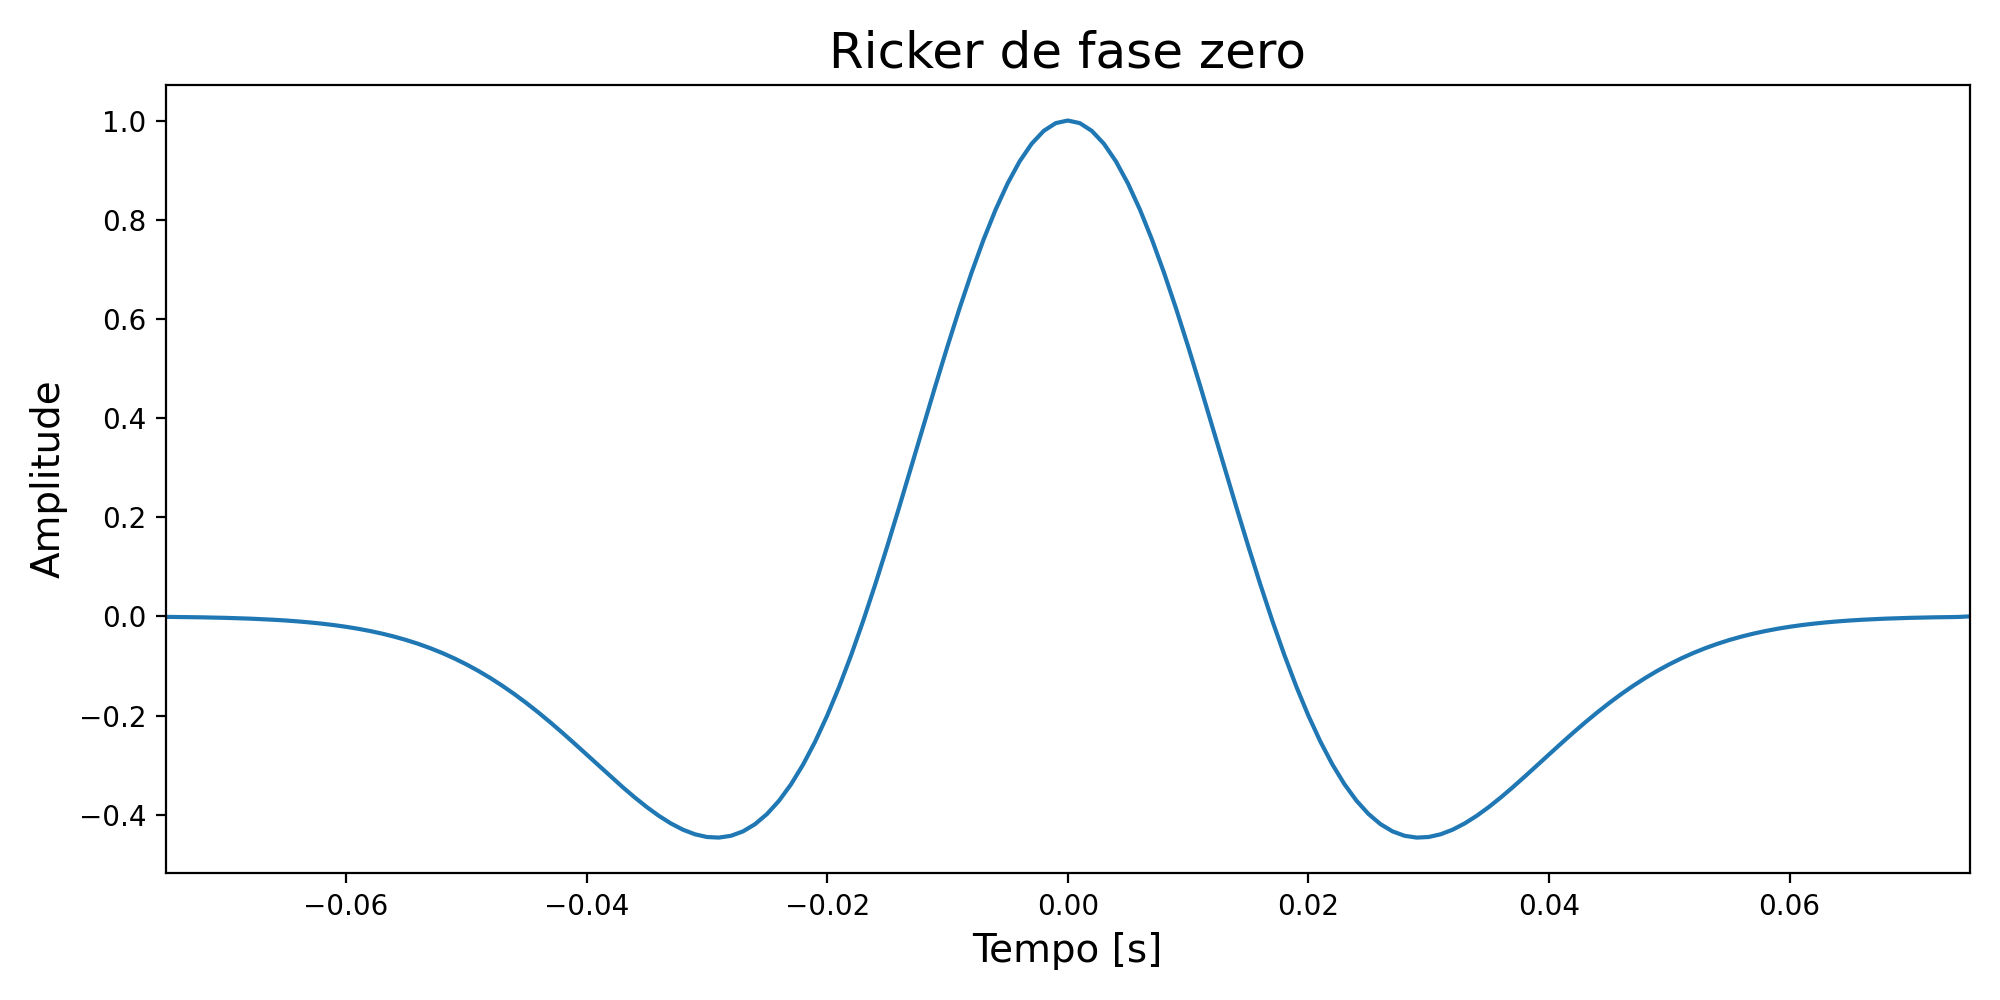
\includegraphics[width=8cm,height=4cm]{Imgs/Metodologia/ricker_zero_phase_a.png}}
	\subfloat[]{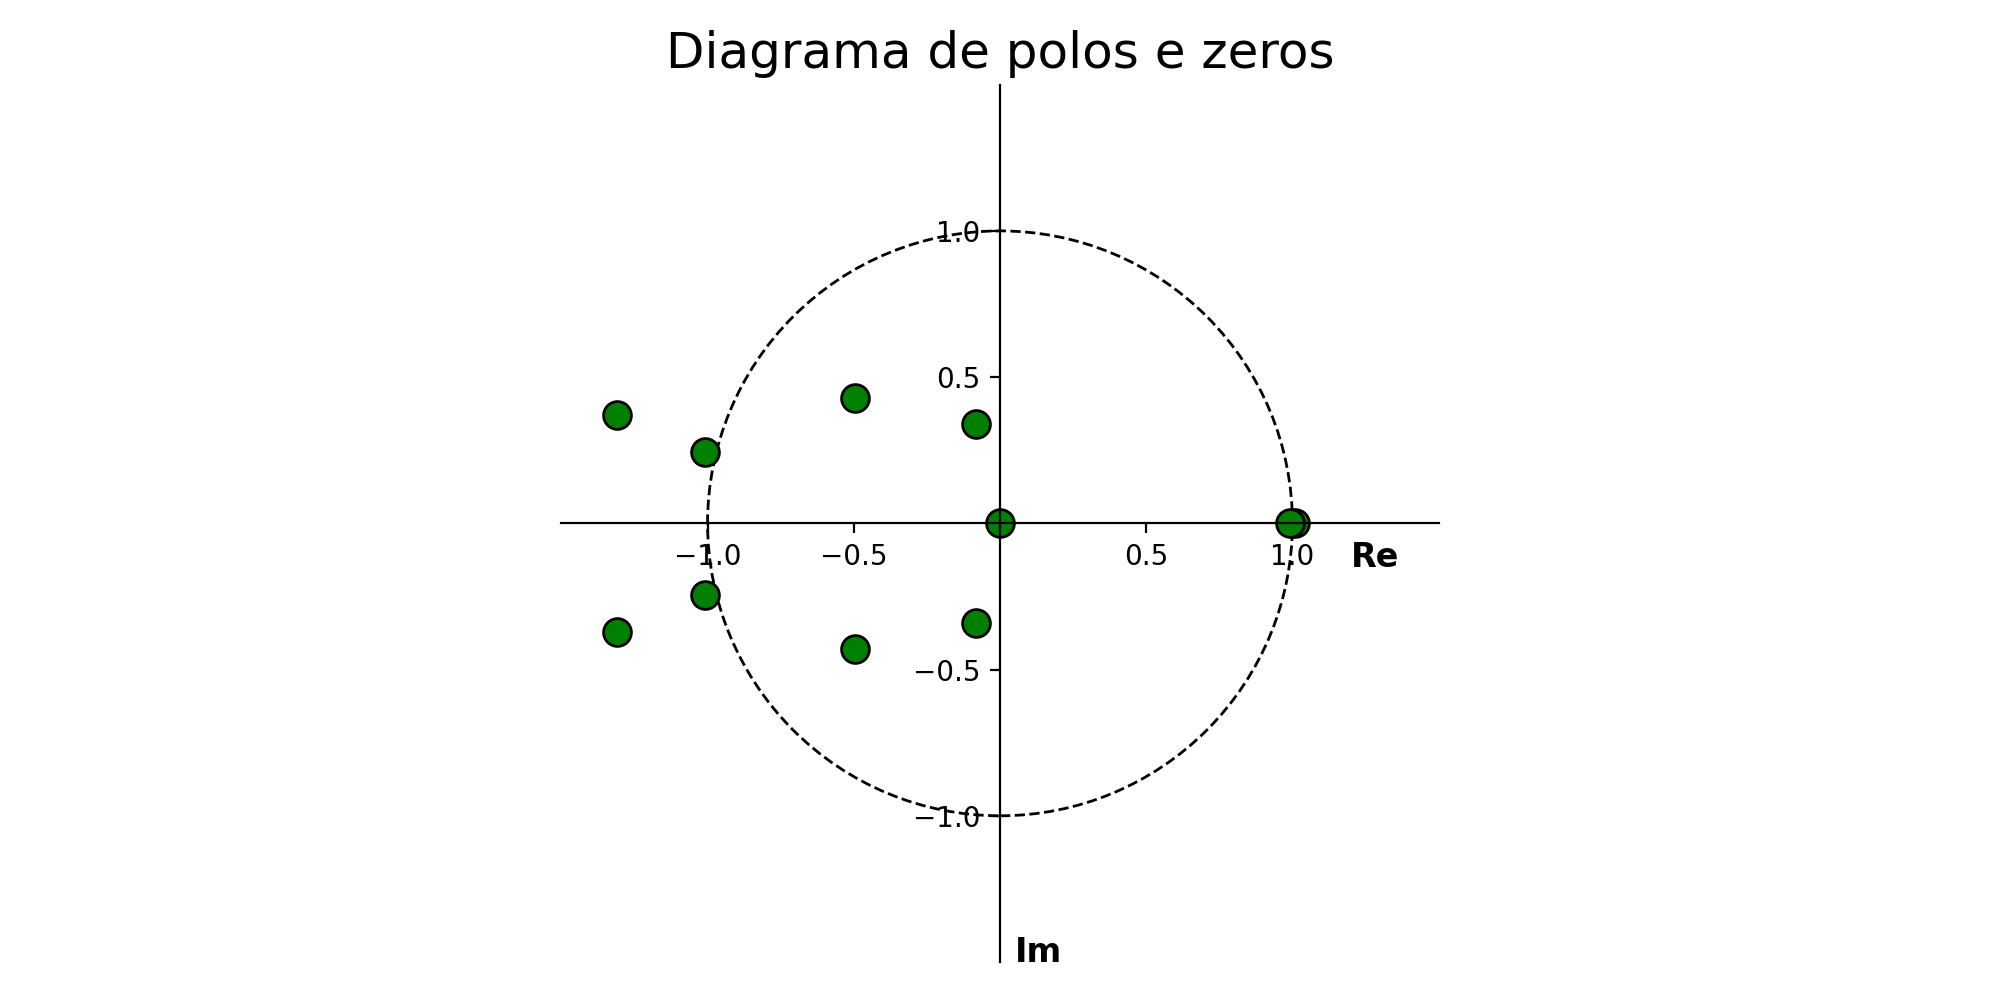
\includegraphics[width=8cm,height=4cm]{Imgs/Metodologia/ricker_zero_phase_b.png}}
	
	\subfloat[]{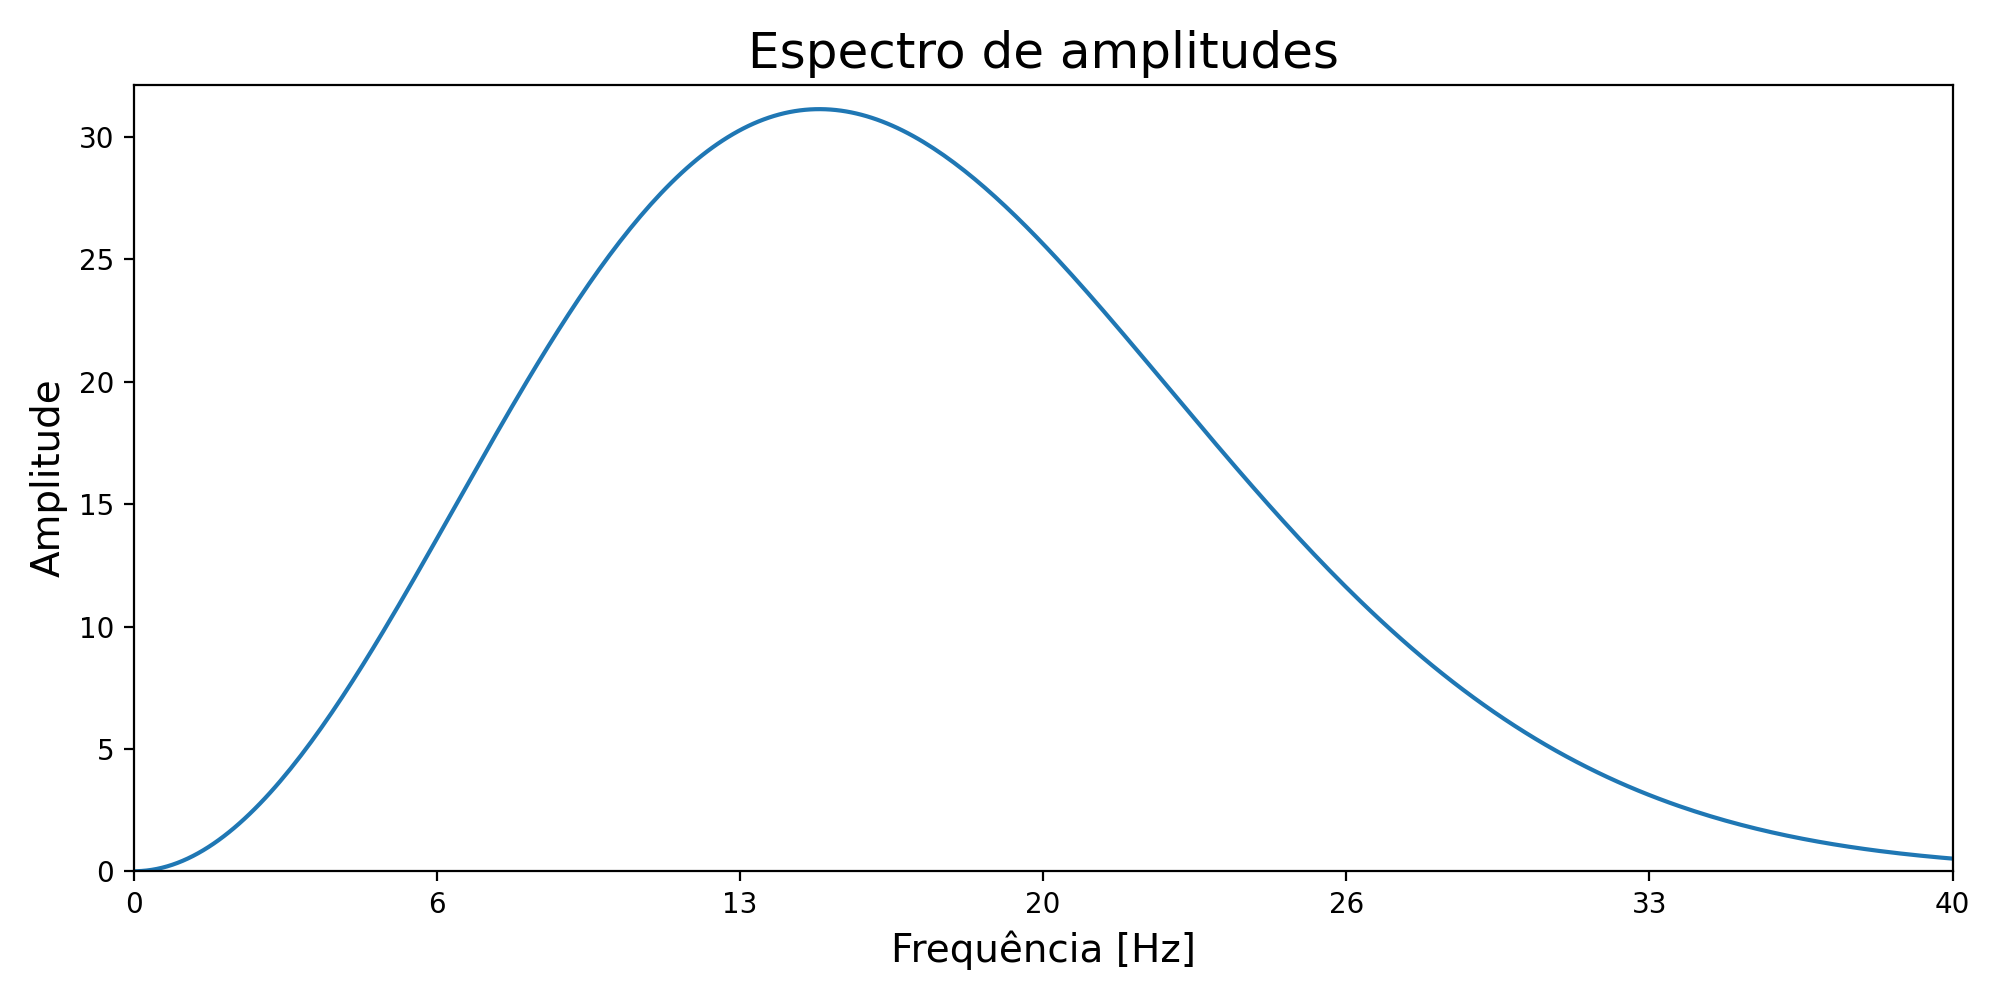
\includegraphics[width=8cm,height=4cm]{Imgs/Metodologia/ricker_zero_phase_c.png}}
	\subfloat[]{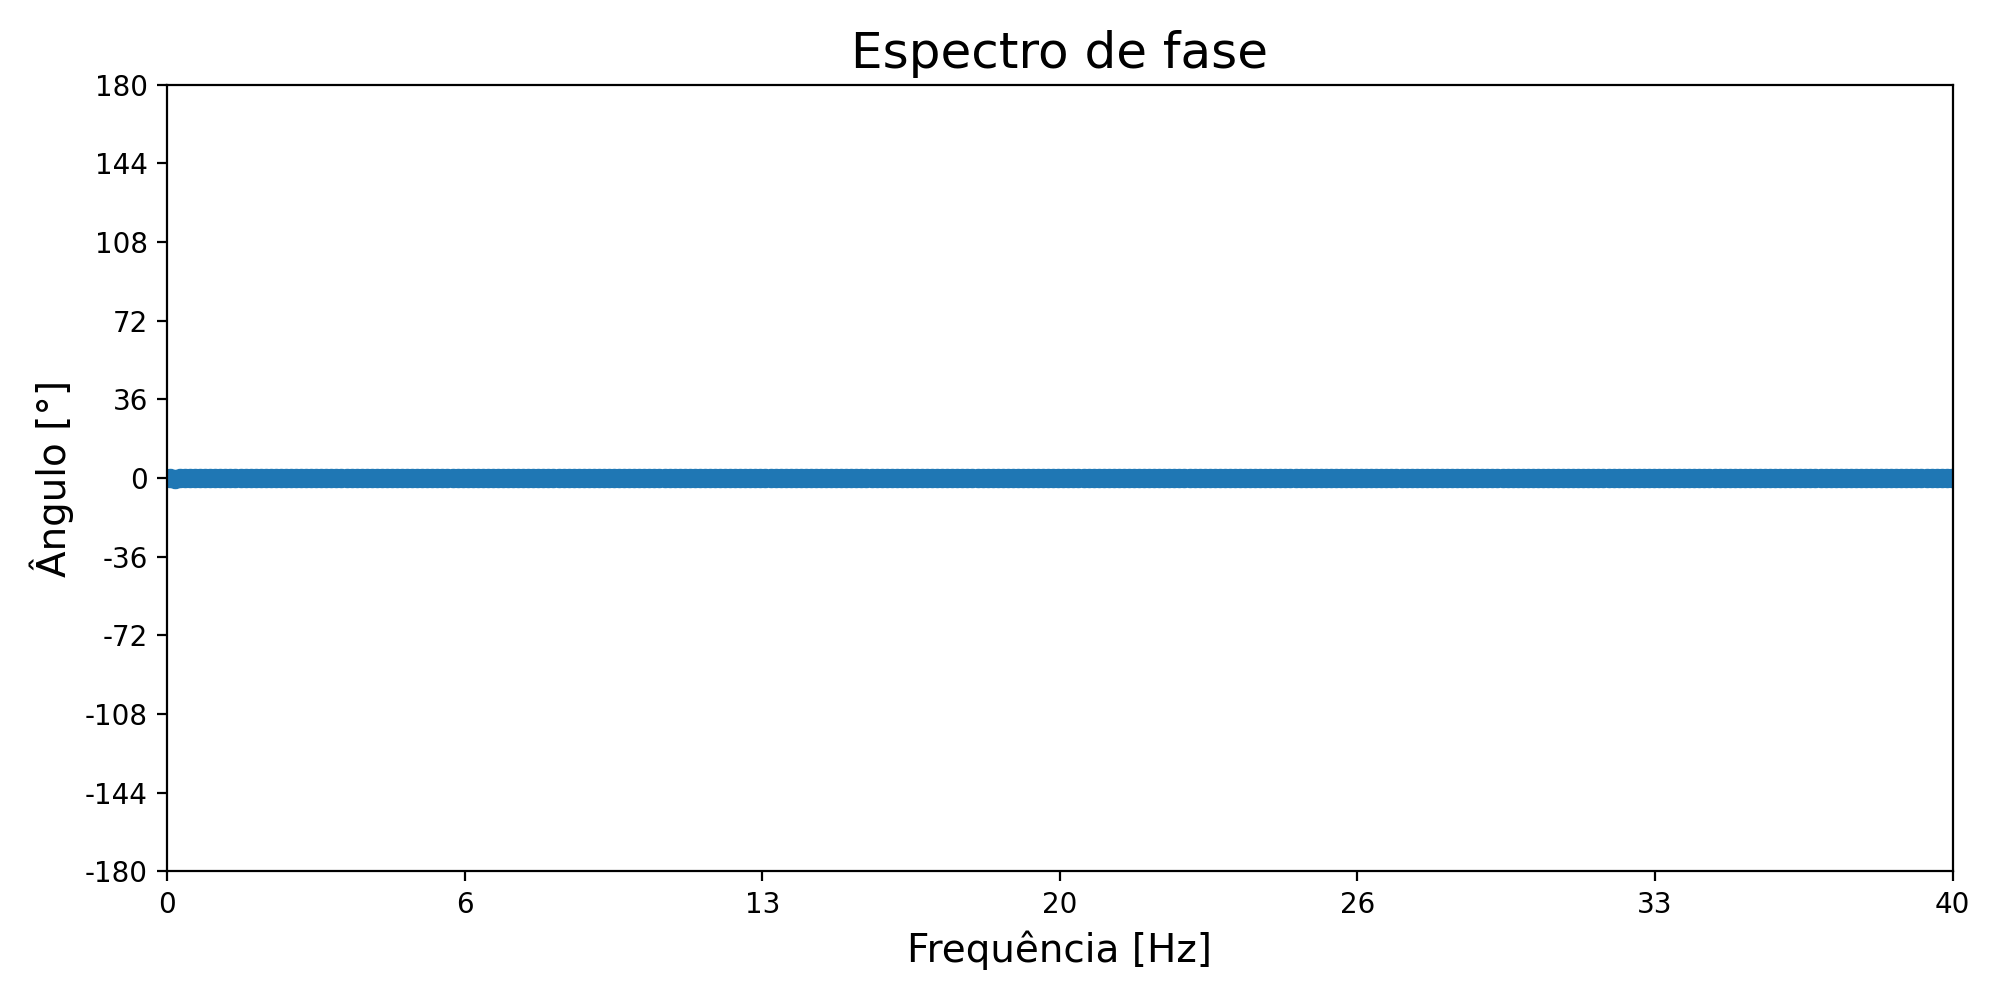
\includegraphics[width=8cm,height=4cm]{Imgs/Metodologia/ricker_zero_phase_d.png}}
		
	\caption{(a) Fonte Ricker centrada em zero. (b) Diagrama de polos e zeros. (c) Espectro de amplitudes e (d) espectro de fase.}
	\label{fig:ricker_zero_phase}
\end{figure}



\begin{figure}[H]
	\centering
	\subfloat[]{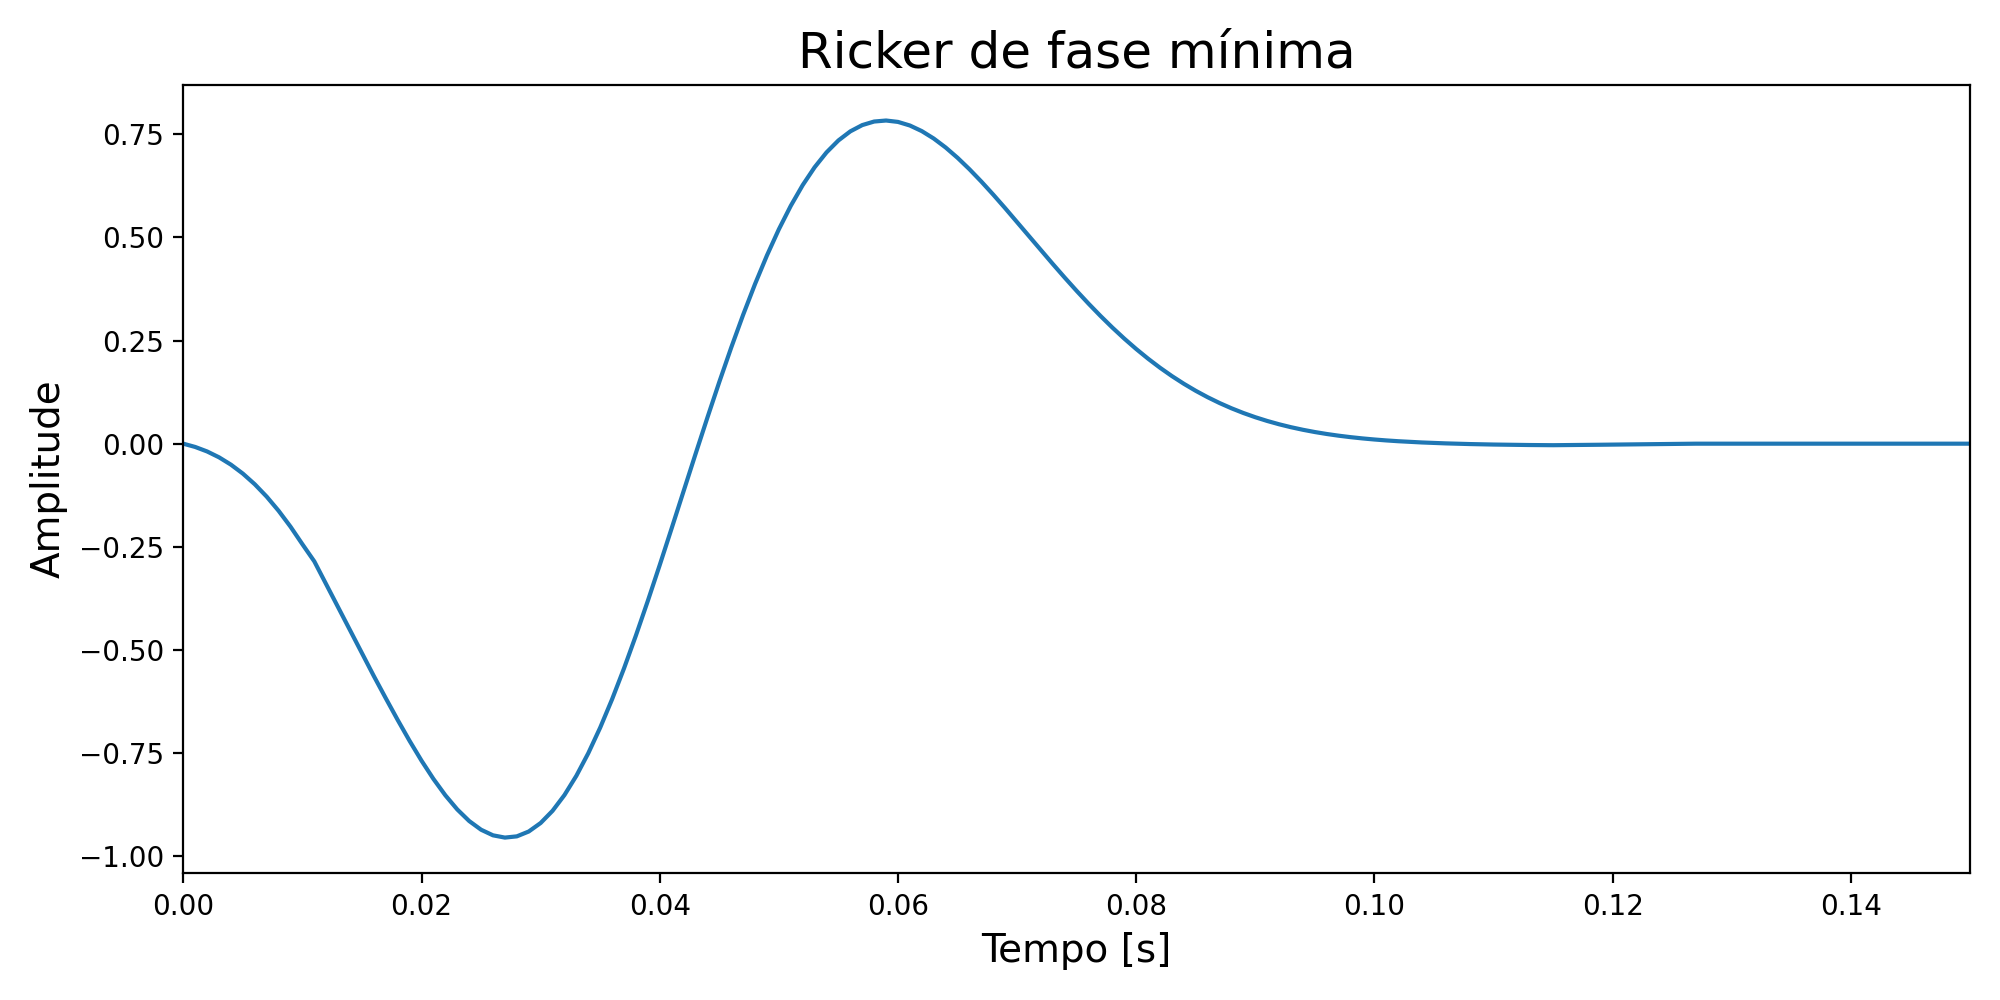
\includegraphics[width=8cm,height=4cm]{Imgs/Metodologia/ricker_min_phase_a.png}}
	\subfloat[]{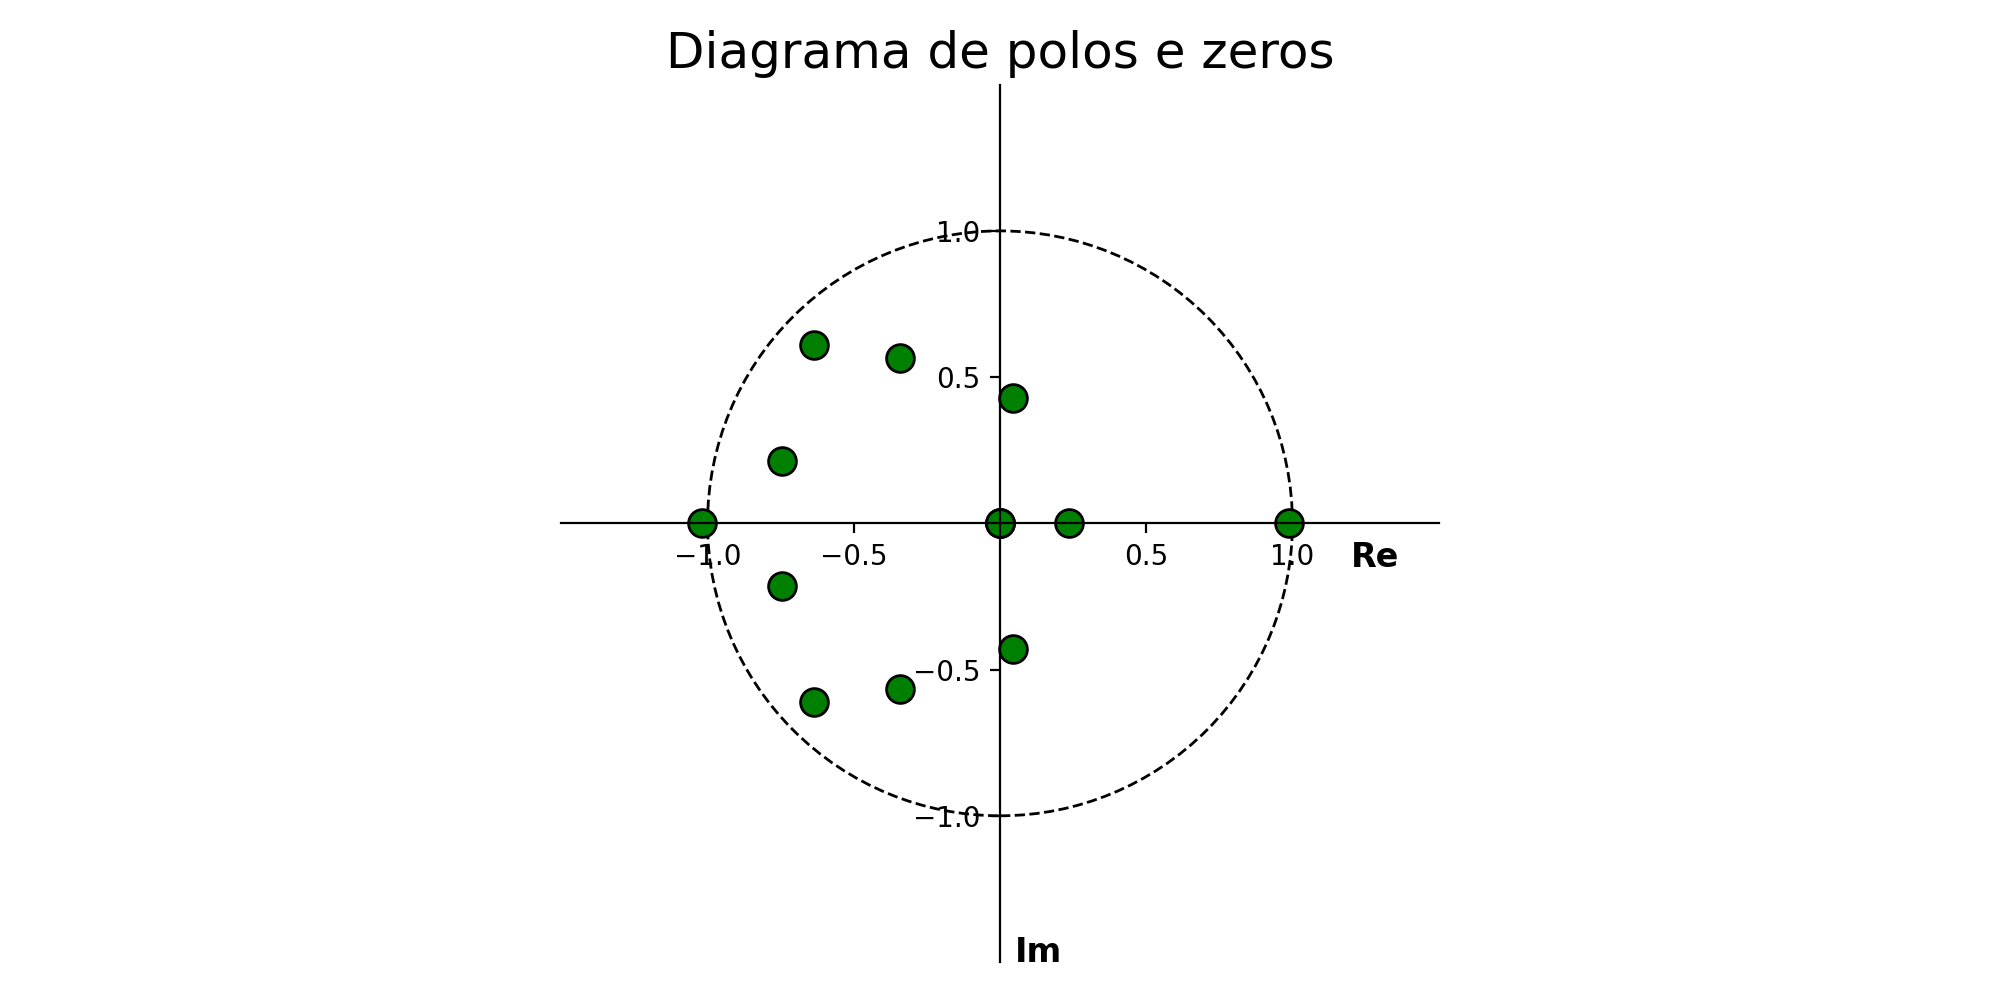
\includegraphics[width=8cm,height=4cm]{Imgs/Metodologia/ricker_min_phase_b.png}}
	
	\subfloat[]{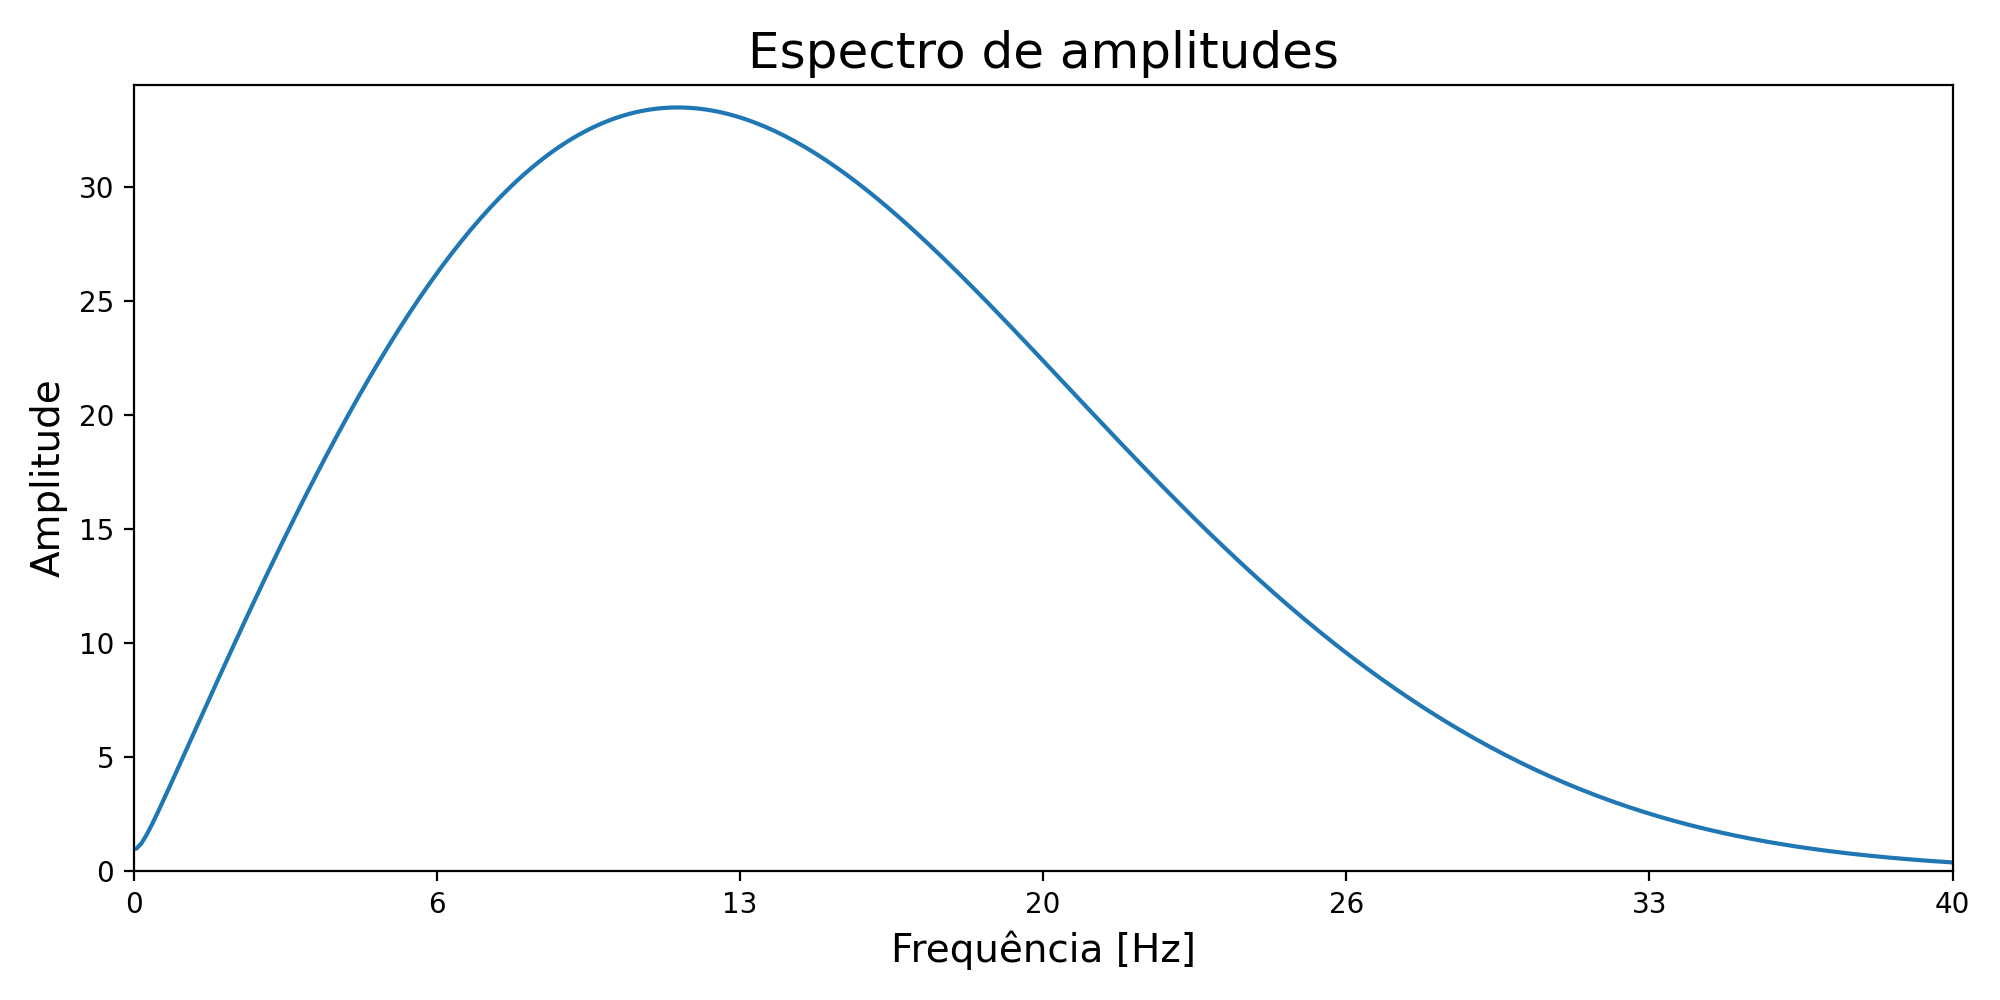
\includegraphics[width=8cm,height=4cm]{Imgs/Metodologia/ricker_min_phase_c.png}}
	\subfloat[]{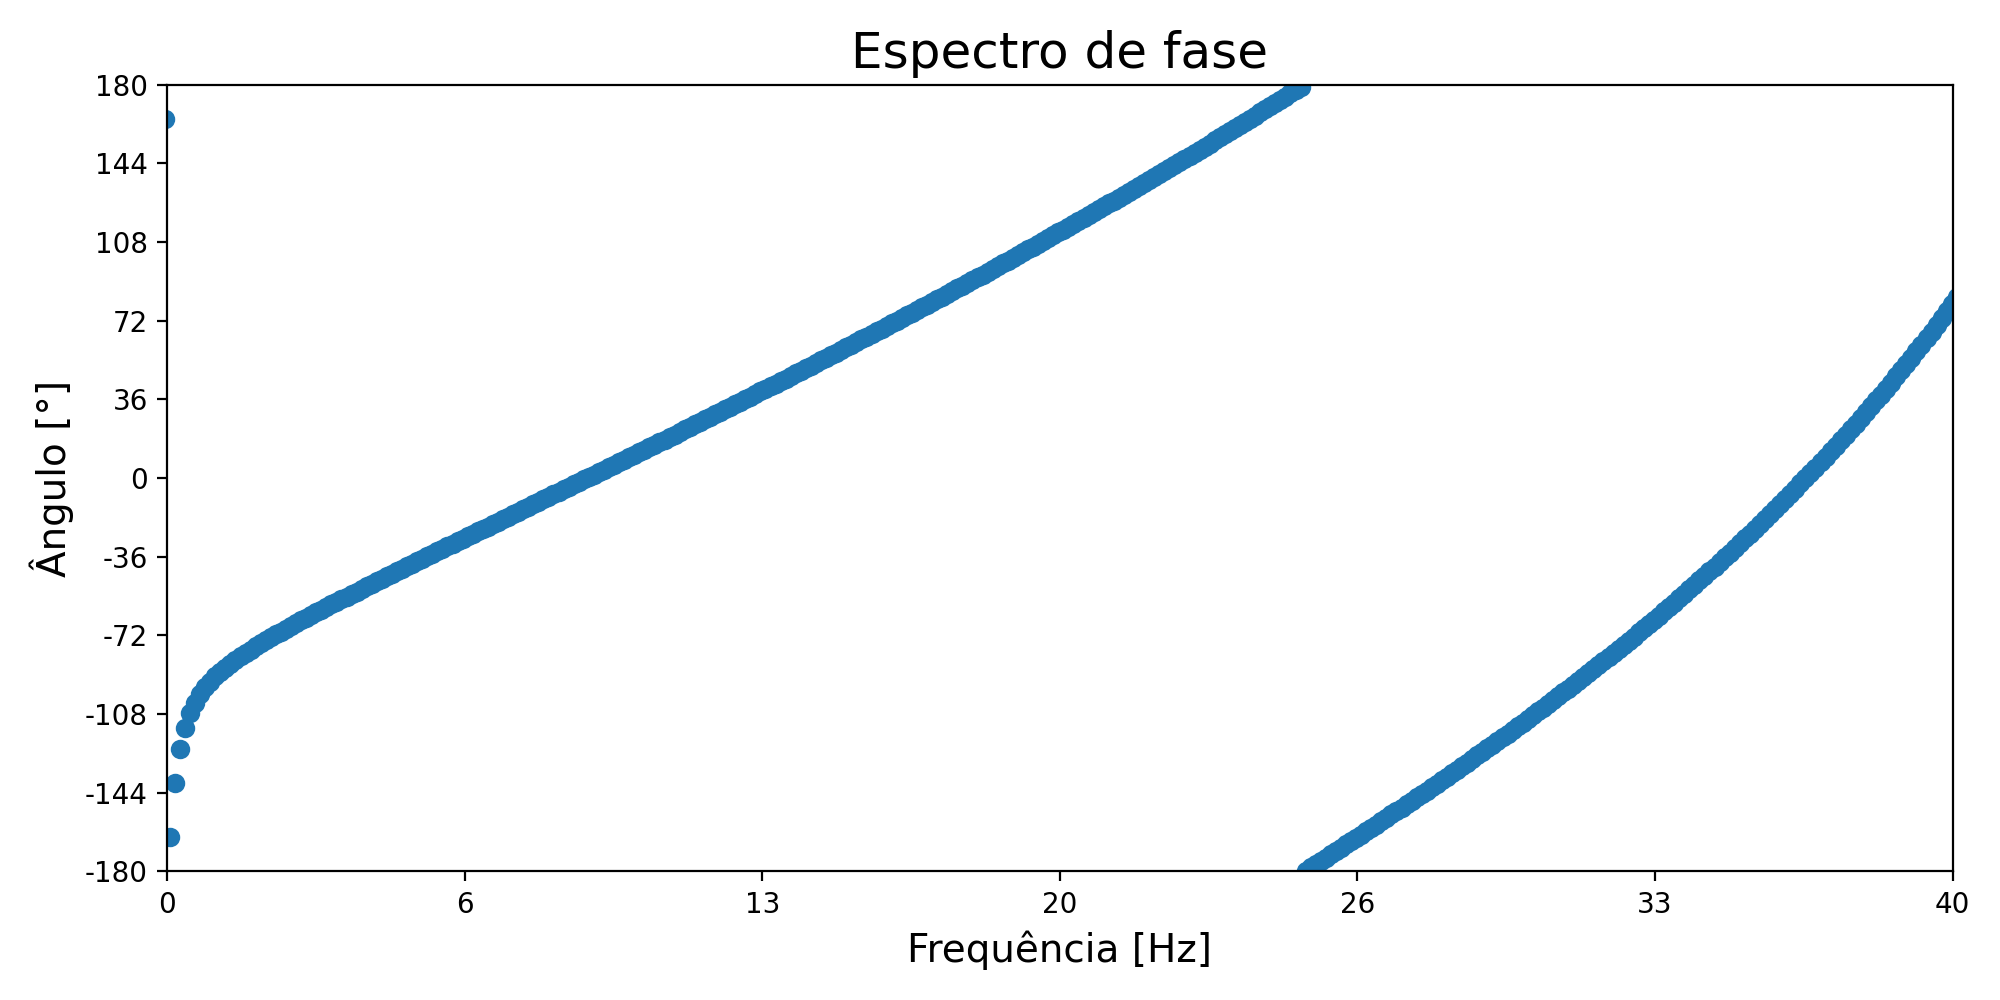
\includegraphics[width=8cm,height=4cm]{Imgs/Metodologia/ricker_min_phase_d.png}}
	
	\caption{Fonte Ricker inicializando de zero. (b) Diagrama de polos e zeros. (c) Espectro de amplitudes e (d) espectro de fase.}
	\label{fig:ricker_min_phase}
\end{figure}


\begin{figure}[H]
	\centering
	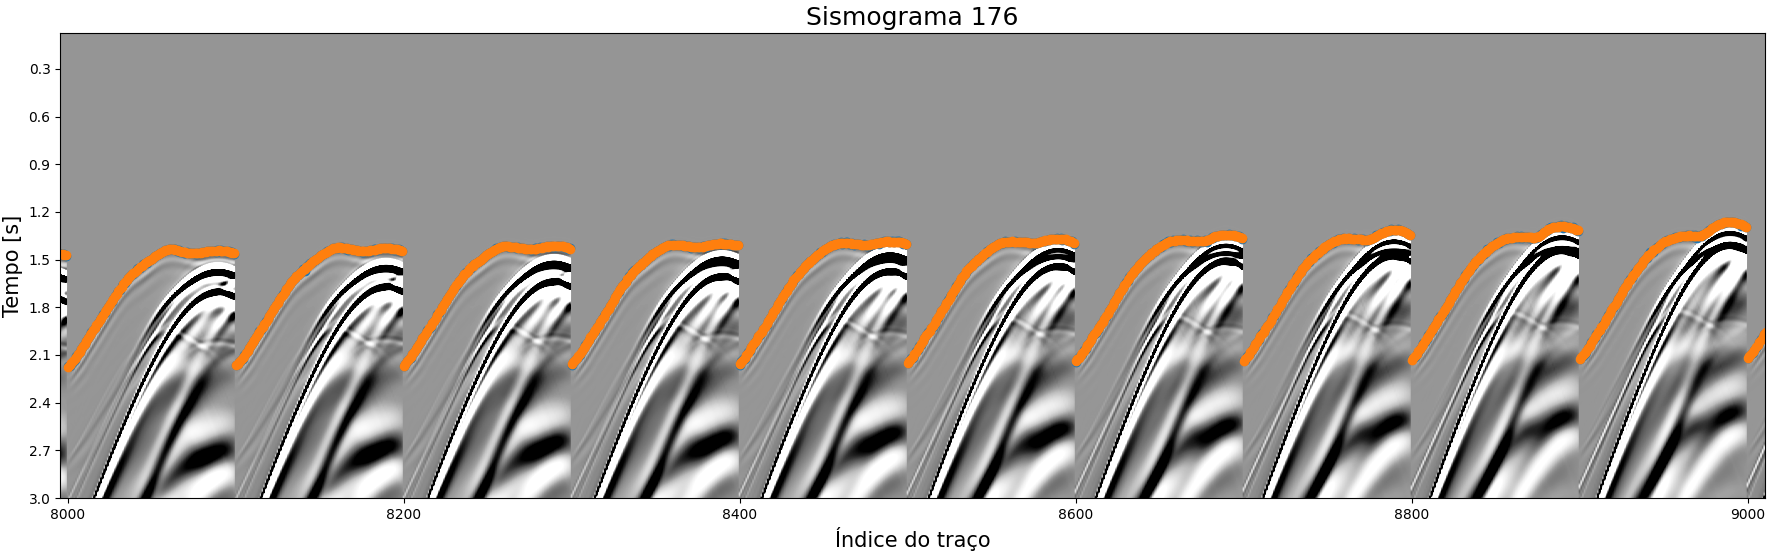
\includegraphics[width=16cm,height=5cm]{Imgs/Metodologia/gather_example.png}
	\caption{Seleção da primeira chegada ilustrada em alguns sismogramas da estação 176.}
	\label{fig:gather_example}	
\end{figure}





\begin{figure}[H]
	\centering
	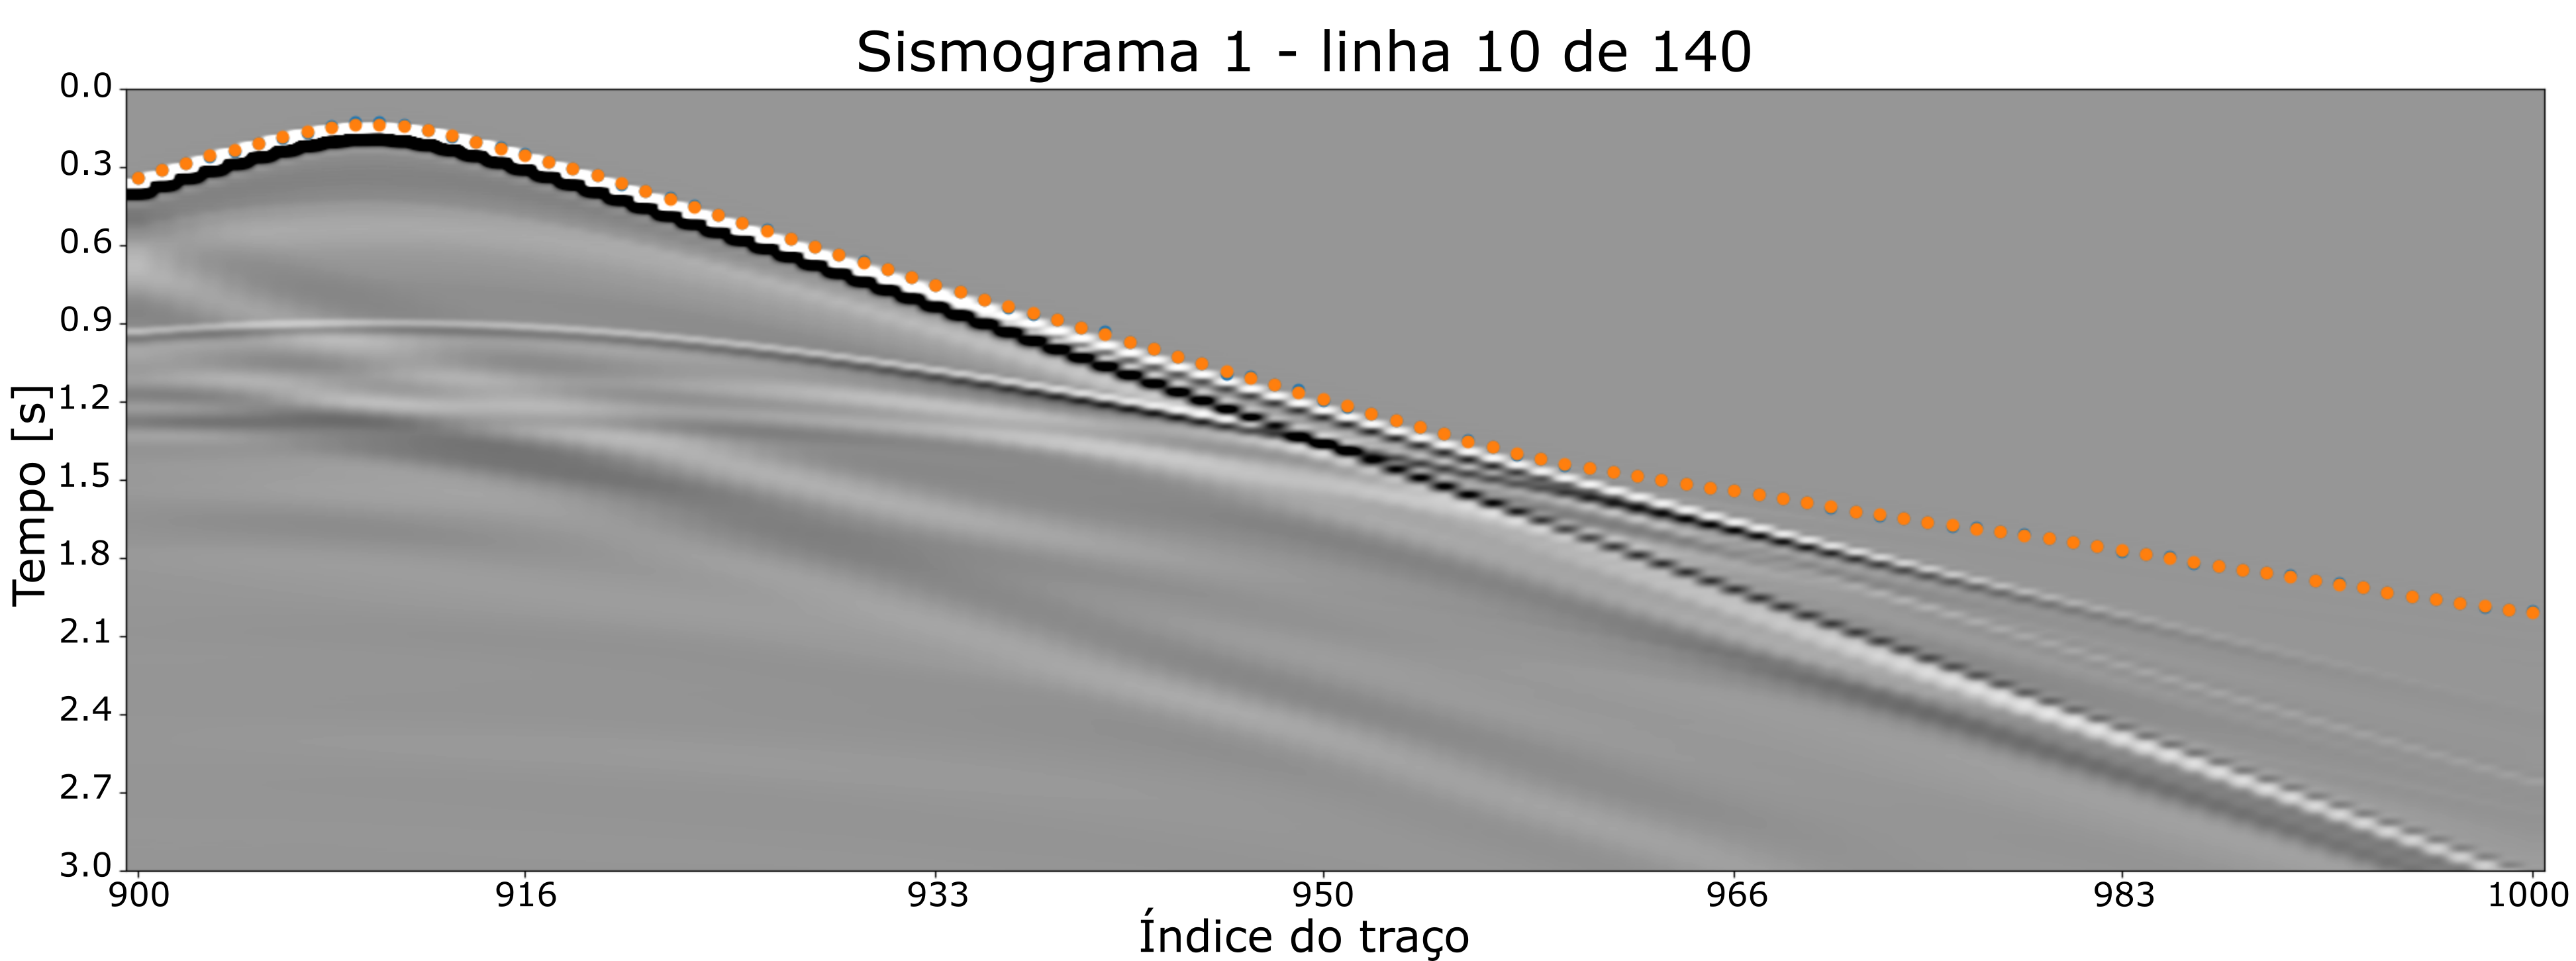
\includegraphics[width=16cm,height=6cm]{Imgs/Metodologia/linha10_sismo1.png}
	\caption{Seleção da primeira chegada em um sismograma de curto afastamento entre fonte e receptor. Presença predominante da onda direta.}
	\label{fig:gather_picking_near}	
\end{figure}

\begin{figure}[H]
	\centering
	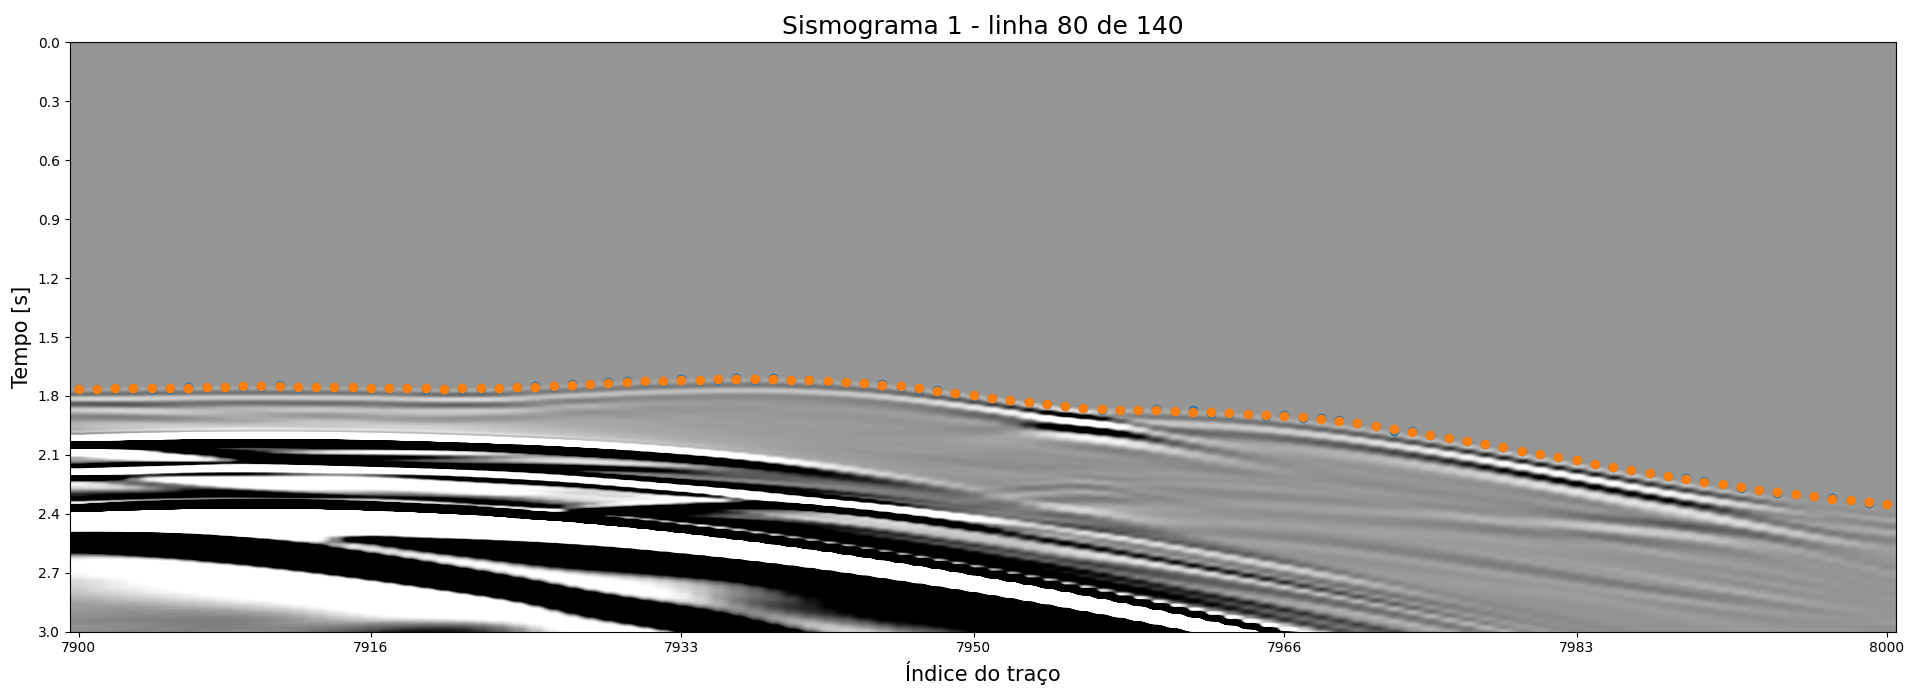
\includegraphics[width=16cm,height=6cm]{Imgs/Metodologia/linha80_sismo1.png}
	\caption{Seleção da primeira chegada em um sismograma de médio afastamento entre fonte e receptor. Presença predominante de refrações.}
	\label{fig:gather_picking_mid}	
\end{figure}

\begin{figure}[H]
	\centering
	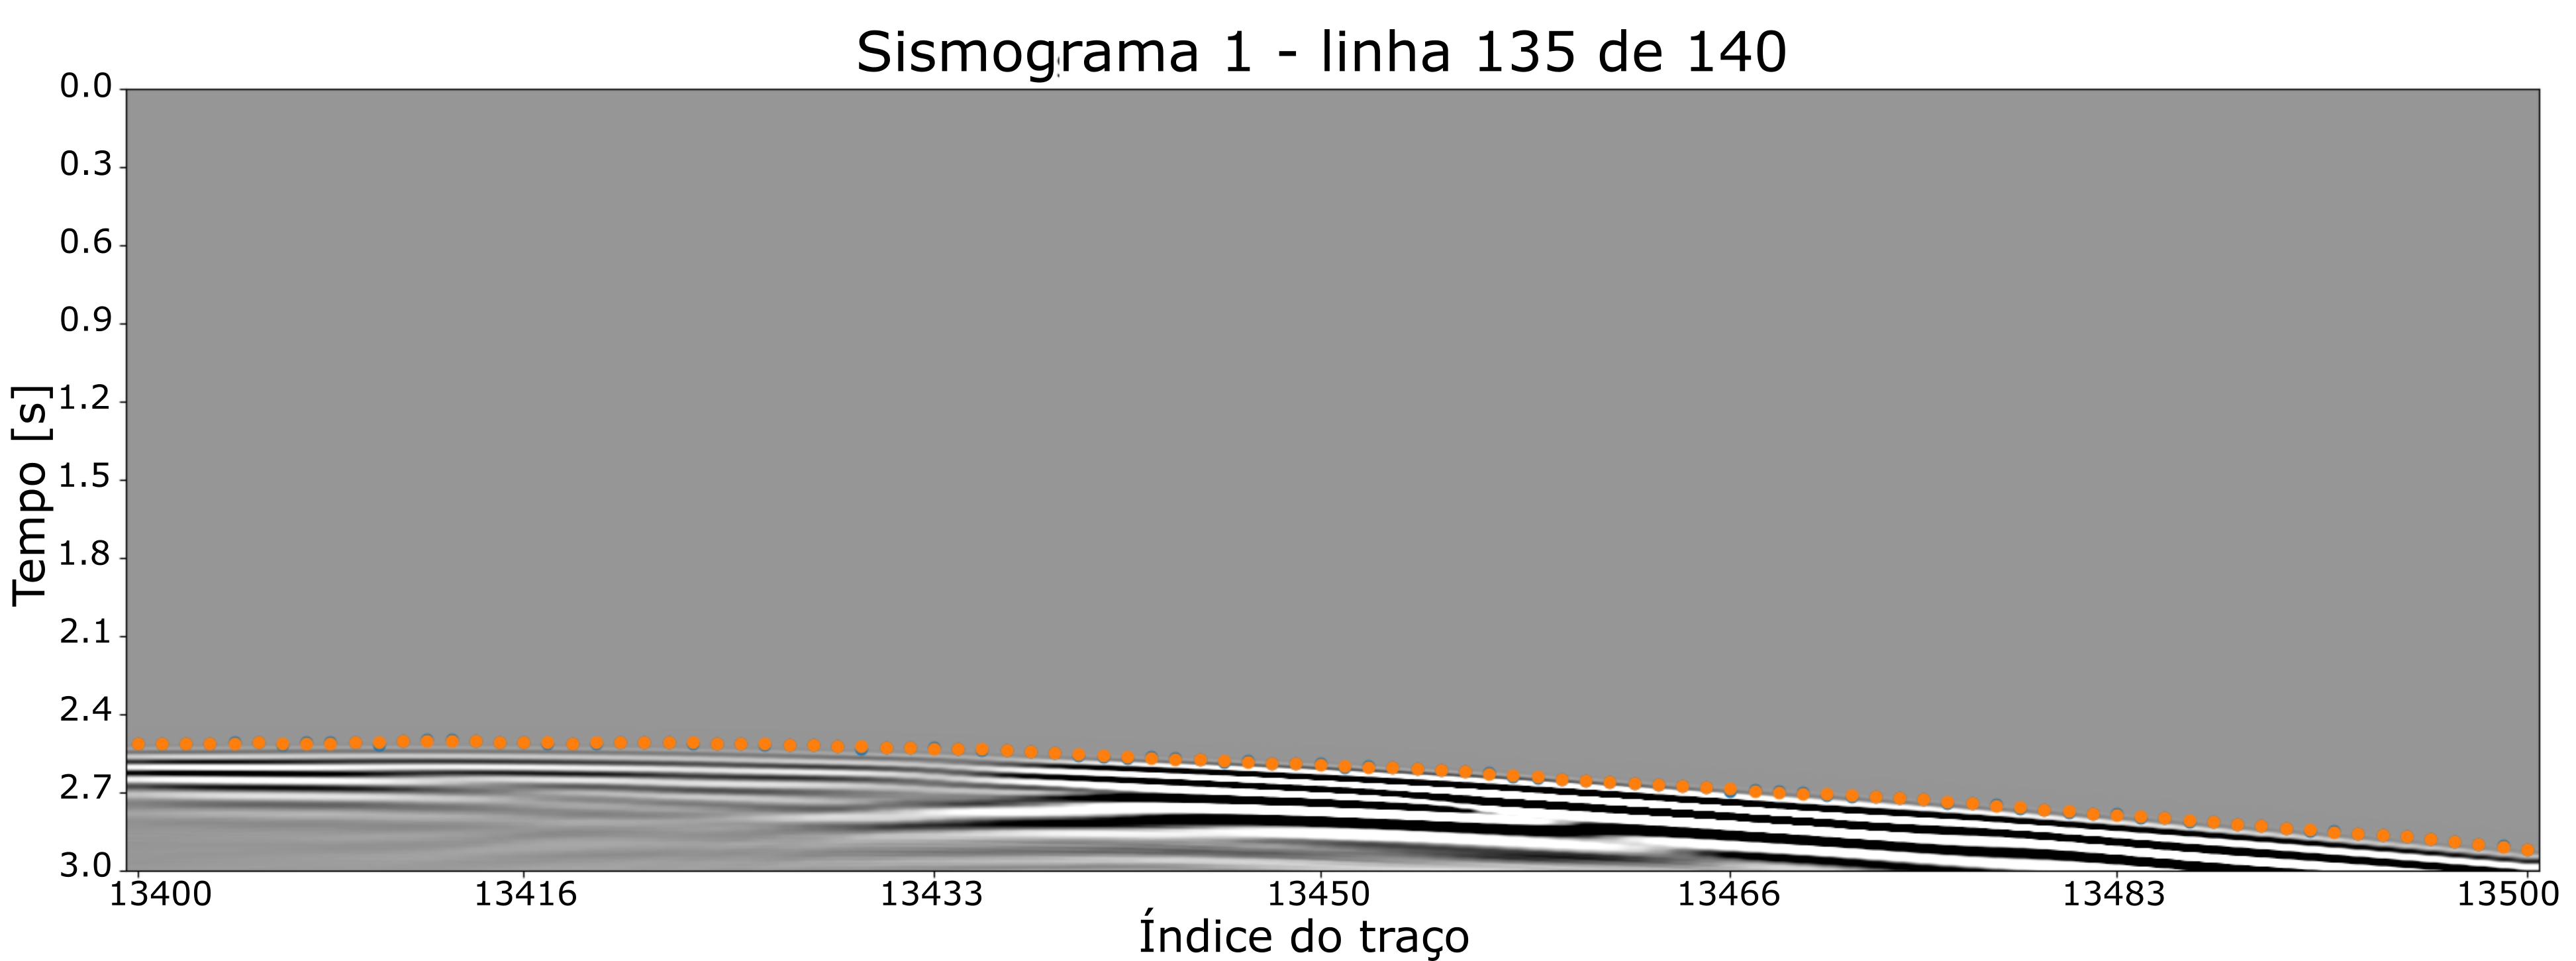
\includegraphics[width=16cm,height=6cm]{Imgs/Metodologia/linha135_sismo1.png}
	\caption{Seleção da primeira chegada em um sismograma de longo afastamento entre fonte e receptor. Somente refrações selecionadas.}
	\label{fig:gather_picking_far}	
\end{figure}




\section{Configurações do esquema de inversão}








